%%%%%%%%%%%%%%%%%%%%%%%%%%%%%%%%%%%%%%%%%%%%%%%%%%%%%%%%%%%%%%%%
%
%  Template for homework of Introduction to Machine Learning.
%
%  Fill in your name, lecture number, lecture date and body
%  of homework as indicated below.
%
%%%%%%%%%%%%%%%%%%%%%%%%%%%%%%%%%%%%%%%%%%%%%%%%%%%%%%%%%%%%%%%%


\documentclass[11pt,letter,notitlepage]{article}
%Mise en page
\usepackage[left=2cm, right=2cm, lines=45, top=0.8in, bottom=0.7in]{geometry}
\usepackage{fancyhdr}
\usepackage{fancybox}
\usepackage{graphicx}
\usepackage{pdfpages} 
\renewcommand{\headrulewidth}{1.5pt}
\renewcommand{\footrulewidth}{1.5pt}
\newcommand\Loadedframemethod{TikZ}
\usepackage[framemethod=\Loadedframemethod]{mdframed}

\usepackage{amssymb,amsmath}
\usepackage{amsthm}
\usepackage{thmtools}
\newtheorem{definition}{Definition}

\usepackage[ruled]{algorithm2e}

\usepackage{afterpage}
%%%%%%%%%%%%%%%%%%%%%%%%
%%%%%% Define math operator %%%%%
%%%%%%%%%%%%%%%%%%%%%%%%
\DeclareMathOperator*{\softmax}{\bf softmax}
\DeclareMathOperator*{\argmin}{\bf argmin}
\DeclareMathOperator*{\argmax}{\bf argmax}
\DeclareMathOperator*{\relint}{\bf relint\,}
\DeclareMathOperator*{\dom}{\bf dom\,}
\DeclareMathOperator*{\intp}{\bf int\,}
%%%%%%%%%%%%%%%%%%%%%%%

\addtocounter{MaxMatrixCols}{11}

\setlength{\topmargin}{0pt}
\setlength{\textheight}{9in}
\setlength{\headheight}{0pt}

\setlength{\oddsidemargin}{0.25in}
\setlength{\textwidth}{6in}
\pagestyle{fancy}
%%%%%%%%%%%%%%%%%%%%%%%%
%% Define the Exercise environment %%
%%%%%%%%%%%%%%%%%%%%%%%%
\mdtheorem[
topline=false,
rightline=false,
leftline=false,
bottomline=false,
leftmargin=-10,
rightmargin=-10
]{exercise}{\textbf{Exercise}}
%%%%%%%%%%%%%%%%%%%%%%%
%% End of the Exercise environment %%
%%%%%%%%%%%%%%%%%%%%%%%

%%%%%%%%%%%%%%%%%%%%%%%
%% Define the Solution Environment %%
%%%%%%%%%%%%%%%%%%%%%%%
\declaretheoremstyle
[
spaceabove=0pt, 
spacebelow=0pt, 
headfont=\normalfont\bfseries,
notefont=\mdseries, 
notebraces={(}{)}, 
headpunct={:\quad}, 
headindent={},
postheadspace={ }, 
postheadspace=4pt, 
bodyfont=\normalfont, 
qed=$\blacksquare$,
preheadhook={\begin{mdframed}[style=myframedstyle]},
	postfoothook=\end{mdframed},
]{mystyle}

\declaretheorem[style=mystyle,title=Solution,numbered=no]{solution}
\mdfdefinestyle{myframedstyle}{%
	topline=false,
	rightline=false,
	leftline=false,
	bottomline=false,
	skipabove=-6ex,
	leftmargin=-10,
	rightmargin=-10}
%%%%%%%%%%%%%%%%%%%%%%%
%% End of the Solution environment %%
%%%%%%%%%%%%%%%%%%%%%%%

%% Homework info.
\newcommand{\posted}{\text{Dec. 9, 2019}}       			%%% FILL IN POST DATE HERE
\newcommand{\due}{\text{Dec. 23, 2019}} 			%%% FILL IN Due DATE HERE
\newcommand{\hwno}{\text{7}} 		           			%%% FILL IN LECTURE NUMBER HERE


\newcommand{\expect}[1]{\text{E} [#1]}
\newcommand{\var}[1]{\text{Var} [#1]}

%%%%%%%%%%%%%%%%%%%%
%% Put your information here %%
%%%%%%%%%%%%%%%%%%%
\newcommand{\name}{\text{Bowen Zhang}}  	          			%%% FILL IN YOUR NAME HERE
\newcommand{\id}{\text{PB17000215}}		       			%%% FILL IN YOUR ID HERE
%%%%%%%%%%%%%%%%%%%%
%% End of the student's info %%
%%%%%%%%%%%%%%%%%%%


\lhead{
	\textbf{\name}
}
\rhead{
	\textbf{\id}
}
\chead{\textbf{
		Homework \hwno
}}


\begin{document}
\vspace*{-4\baselineskip}
\thispagestyle{empty}


\begin{center}
{\bf\large Introduction to Machine Learning}\\
{Fall 2019}\\
University of Science and Technology of China
\end{center}

\noindent
Lecturer: Jie Wang  			 %%% FILL IN LECTURER HERE
\hfill
Homework \hwno             			
\\
Posted: \posted
\hfill
Due: \due
\\
Name: \name             			
\hfill
ID: \id						
\hfill

\noindent
\rule{\textwidth}{2pt}

\medskip





%%%%%%%%%%%%%%%%%%%%%%%%%%%%%%%%%%%%%%%%%%%%%%%%%%%%%%%%%%%%%%%%
%% BODY OF HOMEWORK GOES HERE
%%%%%%%%%%%%%%%%%%%%%%%%%%%%%%%%%%%%%%%%%%%%%%%%%%%%%%%%%%%%%%%%

\textbf{Notice, }to get the full credits, please present your solutions step by step.

\begin{exercise}[Properties of expectation and variance  \textnormal{10pts}]
	Let $X, Y,$ and $Z$ be random variables. Show that the following results hold.
	\begin{enumerate}
	    \item (5pts) The tower property holds, i.e.,
    	\begin{align*}
    	    \expect{X|Y} = \expect{ \expect{X|Y,Z} |Y}.
    	\end{align*}
    	\item (5pts) The variance decomposition formula holds, i.e.,
    	\begin{align*}
    	    \var{X} = \expect{\var{X|Y}}+\var{\expect{X|Y}}.
    	\end{align*}
	\end{enumerate}
    \emph{Hint: if you do not know measure theory well, you can assume that $X$, $Y$, and $Z$ are continuous random variables.}
\end{exercise}


\newpage
\begin{exercise}[Properties of transition matrix \textnormal{30pts}]
    A matrix is nonnegative (positive) if all its entries are nonnegative (positive). A right (left) stochastic matrix is a square nonnegative matrix with each row (column) adds up to one. Without loss of generality, we study the right stochastic matrix in this exercise. Suppose that $T \in \mathbb{R}^{n \times n}$ is a right stochastic matrix.
    \begin{enumerate}
        \item (5pts) Show that $T$ has a eigenvalue 1.
        \item (10pts) Let $\lambda$ be one of $T$'s eigenvalues. Show that $|\lambda|\leq 1$.
        \item (5pts) Show that $I-\gamma T$ is invertable, where $I\in \mathbb{R}^{n\times n}$ is the identity matrix and $\gamma\in(0,1)$.
        \item (10pts) We now show that $(I-\gamma T)^{-1}=\sum_{i=0}^\infty(\gamma T)^i$.
            \begin{enumerate}
                \item For $\mathbf{x}\in\mathbb{R}^n$, we define the infinity norm by
                    \begin{align*}
                        \|\mathbf{x}\|_{\infty}=\max_{i}|x_i|.
                    \end{align*}
                    The induced norm of matrix $M\in\mathbb{R}^{m\times n}$ is
                    \begin{align*}
                        \|M\|_{\infty}=\max_{\|\mathbf{x}\|_{\infty}\leq 1}\|M\mathbf{x}\|_{\infty}.
                    \end{align*}
                        \begin{enumerate}
                            \item Show that $\|M\|_{\infty}=\max_{i}\sum_{j=1}^n|m_{i,j}|$.
                            \item Show that $\|cM\|_{\infty}=|c|\|M\|_{\infty}$ for any $c\in\mathbb{R}$.
                            \item Show that $\|AB\|_{\infty}\leq\|A\|_{\infty}\|B\|_{\infty}$ holds for any $A\in\mathbb{R}^{m\times n}$ and $B\in\mathbb{R}^{n\times p}$.
                        \end{enumerate}
                \item Show that the sequence $I, \gamma T, \sum_{i=0}^2(\gamma T)^2,\dots,\sum_{i=0}^n(\gamma T)^n,\ldots$ is Cauchy. (Hint: a matrix sequence $\{A_p\}$ is Cauchy in $(\mathbb{R}^{m\times n}, \|\, \cdot \, \|_{\infty})$, if given any $\epsilon>0$, there is an integer $N\geq 1$ such that $\| A_p-A_q \|_{\infty}<\epsilon$ whenever $p,q \geq N$.)
                %(Hint: you can use the $\ell_{\infty}$ norm to measure the distance between two matrices.)
                \item Combining the result in the last part and the fact that $\mathbb{R}^{n\times n}$ is complete, we can conclude that $\sum_{i=0}^\infty(\gamma T)^i$ converges to a matrix which we denote by $L$. Show that $(I-\gamma T)^{-1}=L$. (Hint: you need to show that $(I-\gamma T)L=\lim_{n\rightarrow\infty}\sum_{i=0}^{n}(I-\gamma T)(\gamma T)^i$.)
            \end{enumerate}
    \end{enumerate}
\end{exercise}


\newpage
\begin{exercise}[Grid World with a Given Policy \textnormal{30pts}]\label{exercise:GridWorld}

Consider the grid world shown in Figure \ref{fig:gridworld}. The finite state space is $\mathcal{S} = \{s_i:i=1,2,\dots, 11\}$ and the finite action space is $\mathcal{A} = \{\mbox{up, down, left, right}\}$.

\noindent\textbf{State transition probabilities} After the agent picks and performs a certain action, there are four 
possibilities for the next state: the destination state, the current state, the states to the right and left of the current state. If the states are reachable, the corresponding probabilities are 0.8, 0.1, 0.05, and 0.05, respectively; otherwise, the agent stays where it is. The game will terminate if the agent arrives at $s_{10}$ (loss) or $s_{11}$ (win). 
%Once the agent arrives at $s_{10}$ or $s_{11}$, it would stay there forever, i.e., the game is over.

\noindent\textbf{Reward} After the agent picks and performs a certain action at its current state, it receives rewards of 100, -100, and 0, if it arrives at states $s_{11}$, $s_{10}$, and all the other states, respectively.

\noindent\textbf{Policy} In Figure \ref{fig:gridworld}, the arrows show the policy $\pi:\mathcal{S}\rightarrow\mathcal{A}$ for the agent. The random variable $S_t$ is the state at time $t$ under the policy $\pi$. 

\begin{enumerate}
	\item (5pts) Find the matrix $M\in\mathbb{R}^{11\times 11}$ with $m_{i,j}=\mathbf{P}(S_{t+1}=s_i|S_t=s_j)$, i.e., the conditional probability of the agent moving from $s_j$ to $s_i$ .
	
	\item Suppose that the initial state distribution is uniform distribution, that is $\mathbf{P}(S_0=s_i)=1/11$, $i=1,\ldots,11$.
		\begin{enumerate}
		    \item (5pts) Find the distributions $\mathbf{P}(S_1)$ and $\mathbf{P}(S_2)$ by following the policy $\pi$.
			\item\label{exercise:gw-ap} (5pts) Show that the agent would finally arrive at either $s_{10}$ or $s_{11}$, i.e., $$\lim_{t\rightarrow\infty}\mathbf{P}(S_t=s_i)=0,\,i=1,\ldots,9.$$
			\item (5pts) Please find $\lim_{t\rightarrow\infty}\mathbf{P}(S_t=s_{10})$ and $\lim_{t\rightarrow\infty}\mathbf{P}(S_t=s_{11})$.
		\end{enumerate}
	
	\item (5pts) Find the value function corresponding to $\pi$, where the discount factor $\gamma=0.9$.
	
	\item \textbf{Bonus} (10pts) Show that the result in (\ref{exercise:gw-ap}) holds for any initial probabilities we choose for $\mathbf{P}(S_0=s_i)$, $i=1,\ldots,11$.
\end{enumerate}

\end{exercise}

\begin{figure}[h]
	\centering
	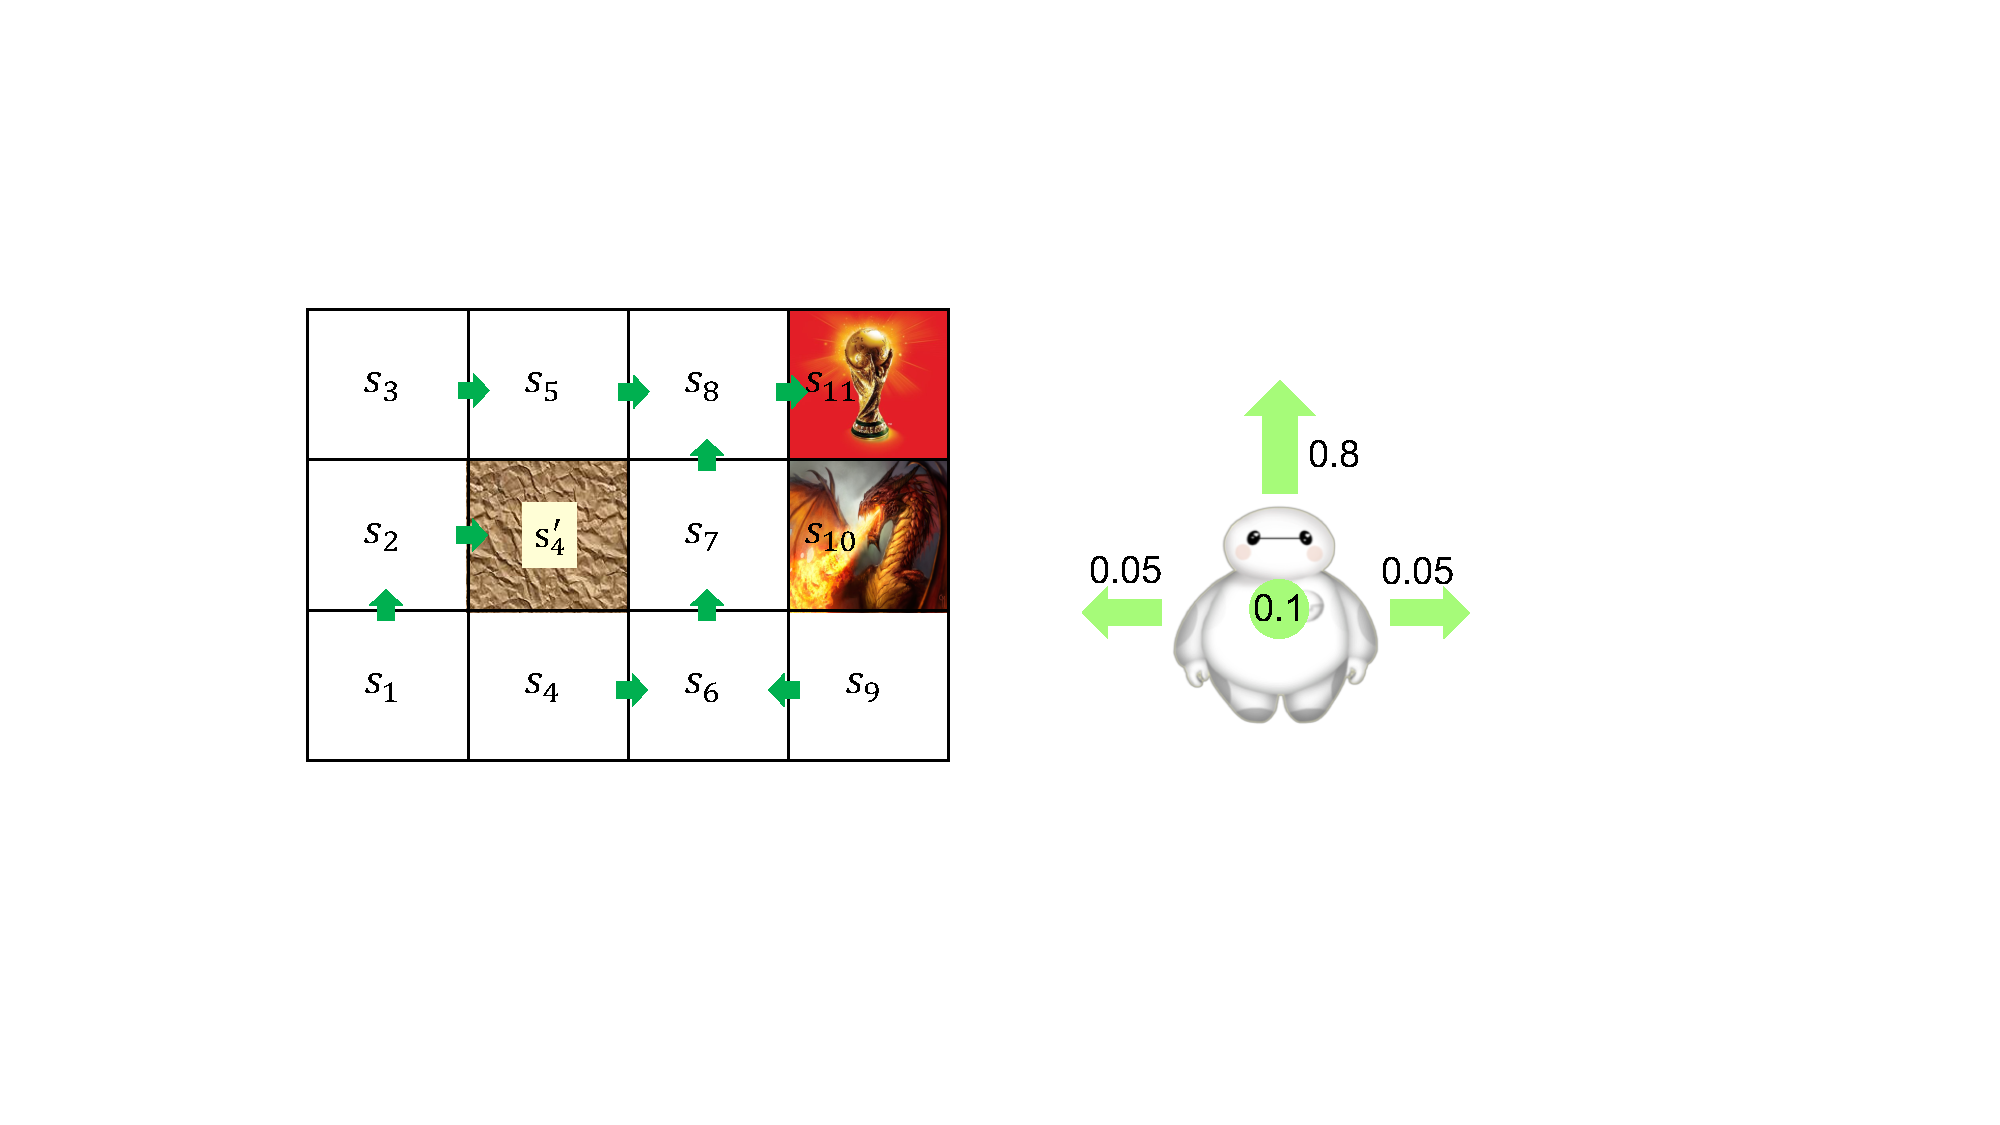
\includegraphics[width=.8\textwidth]{images/Grid_World}
	\caption{Illustration of a grid world with a policy.}\label{fig:gridworld}
\end{figure}



\newpage
\begin{exercise}[Optimal Policy \textnormal{40pts}]
	Consider the grid world problem described in Exercise \ref{exercise:GridWorld}. Let $\pi^*$ be the optimal policy, $V^*$ the corresonding value function, and $\gamma=0.9$. 

	\begin{enumerate}
		\item (10pts) Please derive the Bellman Equation in terms of the value function $V^*$ and the $Q$ function, respectively.
		
		\item (10pts) Please choose one of the algorithms we introduced in class to find $\pi^*$ and $V^*$ respectively and write their pseudocode (hand in your code if you have one).
		
		\item (20pts) Please design a reward scheme such that following the resulting optimal policy will never lose. Specifically, you need to derive the resulting optimal policy and show  $$\lim_{t\rightarrow\infty}\mathbf{P}(S_t=s_i)=0,\,i=1,\ldots,10,$$
		whenever $\mathbf{P}(S_0=s_{10})=\mathbf{P}(S_0=s_{11})=0$.
		%for any $\mathbf{P}(S_0=s_i)$, $i=1,\ldots,9$, and $\mathbf{P}(S_0=s_{10})=\mathbf{P}(S_0=s_{11})=0$.
	\end{enumerate}
	
	
\end{exercise}

\newpage

\begin{exercise}[Policy Iteration \textnormal{20pts}]
    Consider a Markov Decision Process with bounded rewards and finite state-action pairs. The transition probability is $\mathbf{P}[s'|s,a]$ and the reward function is $r(s,a)$. Let $\pi:\mathcal{S}\rightarrow\mathcal{A}$ be a deterministic policy.
    \begin{enumerate}
        \item (10pts) Let $Q^\pi (s,a)$ be the accumulated reward by performing the action $a$ first and then following the policy $\pi$. Find the Bellman Equation for $Q^\pi$.
        \item (10pts) Consider a new policy $\pi'$ given by
        \begin{align*}
            \pi'(s)=\argmax_{a\in\mathcal{A}} Q^\pi(s,a).
        \end{align*}
        Note that if $\argmax_{a\in\mathcal{A}} Q^\pi(s,a)$ is not unique, we can choose one action arbitrarily. Show that  $V^{\pi'}(s) \geq V^\pi(s)$ for all $s\in \mathcal{S}$.
    \end{enumerate}
\end{exercise}





%\newpage
% \bibliography{refs}
%\bibliographystyle{abbrv}

%%%%%%%%%%%%%%%%%%%%%%%%%%%%%%%%%%%%%%%%%%%%%%%%%%%%%%%%%%%%%%%%

\end{document}
